% !TEX root = ../my-thesis.tex
%
\chapter{Discussion}\label{sec:discussion}
After the models have been calculated, the next step is to critically examine and evaluate the results. The evaluation of the spatial models follows a simple scheme. First, a brief look is taken at the models without the spatial component, before the spatial models are reviewed and compared with the non-spatial models. Next, it is examined which factors significantly influence the risk of infection and why these factors might have an impact. For this, the coefficient of the BYM2 model are analysed. Finally, a look at area-specific risk is taken to see which regions in a given country are most at risk.
\section{Discussion of the (Non)-Spatial Models}
\subsection{Discussion of the (Non)-Spatial Models for Norway}\label{sec:models_norway}
The non-spatial model for Norway identified five significant effects:
\begin{itemize}
    \item The number of unemployed immigrants 
    \item The total number of immigrants 
    \item The urban density 
    \item The number of aerodromes 
    \item The proportion of females 
\end{itemize}
Moreover, the intercept was significant. \\
Comparing the spatial models with the non-spatial models using Table~\ref{allNorway}, it can be seen that BYM2, Besag and the non-spatial model performed almost equally well in terms of the DIC and WAIC, while the Leroux model performed best in terms of these two metrics. In terms of CPO, all spatial models performed better than the non-spatial model, with the Leroux model again performing best. However, the MAE shows that the non-spatial model has the best predictive performance, ahead of the Besag model, the BYM2 model and the Leroux model. This shows that the Leroux model overfits the training data more than the other models, a characteristic that can also be seen in Figure~\ref{comparison_norway_1} and Figure~\ref{comparison_norway_2}. The fact that the non-spatial model performs better than the spatial models is an indication that the spatial effect in Norway is not strong and that a different class of models may be better suited to identify critical factors affecting infection rates. Table~\ref{fixedAllNorway_spatial} also shows that adding the spatial effect did not suddenly cause any variables to become significant, while all variables, including the intercept, that were significant in the non-spatial model remained significant. Nevertheless, significant effects were found and have to be discussed. \\
The exponentiated intercept implies a risk rate of -60.8\% across Norway. The factor that influences the relative risk most is urban density, where an increase of 1 standard deviation leads to an increase in the relative risk of 22.5\%. The relationship between a higher number of residential buildings in a given area and the number of infections is probably due to the fact that with an increasing number of residential buildings comes an increasing number of inhabitants. A look at the Bravais-Pearson correlation coefficient confirms this assumption with $\rho=0.7070$. Furthermore, the correlation between urban density and population density is $0.8037$. This is convenient since studies analysing the relationship between urban density and Covid-19 usually define urban density as the number of inhabitants per square kilometre. Because of the positive relationship between urban density and population density, urban density acts as a proxy for population density in these models, so the relationship between higher population density and higher case numbers should also account for the higher infection rates in areas with higher urban density. According to Jamshidi et al. (2020) and Whittle \& Diaz-Artiles (2020), higher urban/population density and higher infection numbers are due to a decrease in proximity between people and an increase in the likelihood of interpersonal contact (Jamshidi2020global, Whittle2020ecological). Sigler et al. (2020) also found that dense urban environments provide more opportunities for the virus to spread, but that higher density had a stronger effect earlier and decreased in strength and importance over time\autocite[][]{sigler2020socio}. \\
Factors related to immigration also play a crucial role in the relative risk of developing Covid-19. A one standard deviation increase in the number of unemployed immigrants leads to a 20.8\% increase in risk and a one standard deviation increase in the total number of immigrants leads to a 20.3\% increase in risk. Unfortunately, there are no studies analysing the relationship between unemployed immigrants and the risk of developing Covid-19, as studies mostly focus on the relationship between unemployment in general and the risk of disease. Unemployment, however, turned out to be non-significant in the BYM2 model. Looking at older studies, Elkeles and Seifert (1996) conducted a longitudinal study that looked at the unemployment status and health of labour migrants in Germany. They found that immigrants were often employed in jobs with higher health risks and stress and therefore had poorer health \autocite[][]{elkeles1996immigrants}. Sia et al. (2019) analysed the association between immigration status and unemployment and men's and women's health using data from the Canadian Health Measures Survey. The study provided evidence of biological associations between unemployment and the likelihood of common chronic diseases, inflammation and possible malnutrition, with unemployed immigrants, and particularly unemployed immigrant women, being more prone to chronic diseases \autocite[][]{sia2019chronic}. Thus, there is precedent for an association between unemployment and immigrants and a higher risk of disease, however, further research would need to be conducted to analyse the association between unemployed immigrants and the risk of Covid-19 infection. \\
A higher risk among immigrants in Norway was already found in a study by Indseth et al. (2020). The reasons given are barriers to adequate information due to low health literacy in certain groups and misconceptions about Covid-19 or test criteria, as well as other socio-economic and environmental factors \autocite[][]{indseth2020covid}. Therefore, the results of the BYM2 model are consistent with this study. \\
Looking at the factors that reduce the risk of infection for Covid-19, for airports, a 1 standard deviation increase leads to a 12.2\% reduction in risk and a 1 standard deviation increase in the proportion of women leads to an 18.2\% reduction in the risk of infection. Neither result is consistent with current research. Gaskin et al. (2021) found that counties in the United States closer to an airport have higher Covid-19 rates than counties further from an airport \autocite[][]{gaskin2021geographic}. Daon et al. (2020) found that different airports have different risks of being a source of an outbreak, especially airports in low- to middle-income countries \autocite[][]{daon2020estimating}. \\
Many studies have investigated the relationship between gender and Covid-19 and most come to the same conclusion. While the risk of infection is the same in men and women, men tend to experience a higher severity and mortality rate for Covid-19 compared to women \autocite[][]{mukherjee2021covid, gausman2020sex, spagnolo2020sex, kopel2020racial}. \\
A look at the relative risk of infection in Figure~\ref{rr_norway} shows that the relative risk is below 1 in most of Norway, which is not too surprising considering that Norway has managed the pandemic quite well so far. The two municipalities with the highest relative risk are Iveland and Ålesund. However, a look at the posterior probability in Figure~\ref{posterior_norway} shows that the posterior probability of the risk being greater than 1 is less than 0.5 for Ålesund (0.47) and less than 0.75 for Iveland (0.62). Looking at the log posterior mean of the random effects, there is an increased risk in the regions around Oslo and in large parts of southern and central Norway, while the risk tends to be lower in the northern parts of the country.
\begin{figure}[H]
  \centering
  \includegraphics[width = \textwidth]{relative_risk_norway.png}
  \caption{Relative risk of contracting Covid-19 in Norway.}
  \label{rr_norway}
\end{figure}
\begin{figure}[H]
  \centering
  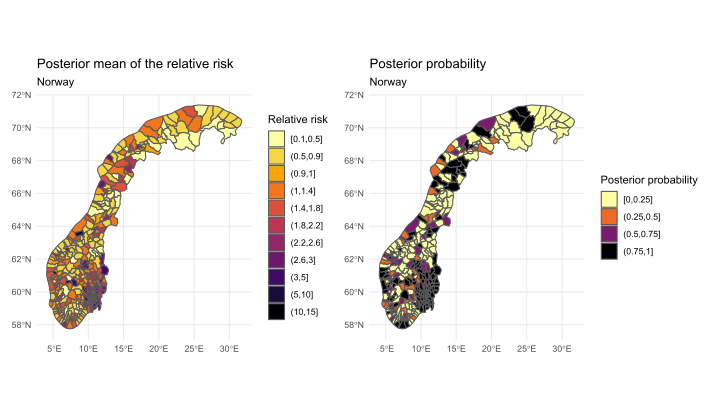
\includegraphics[width = \textwidth]{posterior_norway.png}
  \caption{Posterior mean of the municipality-specific relative risks $\zeta=\exp{\left(\xi\right)}$ compared with the whole of Norway (left) and posterior probability $\mathbb{P}\left(\zeta_i>1|\pmb{y}\right)$}
  \label{posterior_norway}
\end{figure}
\subsection{Discussion of the (Non)-Spatial Models for Germany}
In the non-spatial model for Germany, six coefficients were significant, in addition to the intercept:
\begin{itemize}
    \item The percentage of the vote for the right-wing populist AfD
    \item The population density
    \item The logarithmic trade tax
    \item The percentage of the vote for the SPD
    \item The percentage of the vote for the left-wing party "Die Linke"
    \item The percentage of the vote for the Green party
\end{itemize}
A look at Table~\ref{allGermany} shows that the spatial models outperform the non-spatial model in terms of the DIC and the WAIC, while all models perform about equally well in terms of the CPO. The predictive performance was best for the BYM2 model, just ahead of the Besag model, as indicated by the lowest values for the MAE. When adding the spatial term for the BYM2 model, several variables lose their significance, namely the percentage of the vote for the SPD, "Die Linke" and the Greens, while the intercept, the percentage of the vote for the AfD, population density and the logarithmic trade tax remain significant. \\
The exponentiated intercept implies a risk rate of -6.8\% across Germany. The greatest influence on the relative risk was determined to be the percentage of the vote for the far-right AfD. An increase in this variable by 1 standard deviation leads to an increase in the relative risk by 24.8\%. The AfD openly criticises the measures taken by the government in Germany to prevent the spread of Covid-19, which leads to a large proportion of the party's voters not taking the measures seriously and refusing to keep a safe distance or wear a mask in public spaces. Several studies have taken a look at the response of right-wing parties to the pandemic and how people who vote for these types of parties have reacted. Wondreys and Mudde (2020) point out that these parties were quick to warn about the virus, but once cases spiked, they criticised the measures taken to contain the spread of the virus. They also noted that right-wing parties often rejected the measures proposed by the leading parties because they themselves were part of the opposition \autocite[][]{wondreys2020victims}, as is the case with the AfD in Germany. Vieten (2020) shows how the far-right mobilises people for anti-hygiene or anti-lockdown protests and how this is used to normalise the global far-right \autocite[][]{vieten2020new}. Eberl et al. (2020) analysed data from the Austrian Corona Panel Project to test whether populism attitudes and belief in conspiracy theories related to Covid-19 are correlated. Using structural equation modelling, they show that populism indirectly influences Covid-19 conspiracy beliefs through trust in political and scientific institutions. They find that populist attitudes have a negative correlation with trust in the government and the parliament.Furthermore, they find that higher populist attitudes are negatively correlated with trust in science, a factor that reduces belief in Covid-19 conspiracy theories \autocite[][]{eberl2020populism}. Finally, Farias and Pilati (2020) conducted a study in Brazil to predict social distancing violation intention and past non-compliance during the Covid-19 pandemic, controlling for the effects of interolerence of insecurity and socio-demographic variables. Their results included that individuals who support right-wing parties are more likely to violate social distancing measures \autocite[][]{farias2020violating}. \\
An increase in population density by 1 standard deviation leads to a risk increase of 11.2\%. Reasons why a higher population density correlates positively with the number of infections have already been discussed in Section~\ref{sec:models_norway}. \\
The last significant effect is the logarithmic trade tax with an increase of 1 standard deviation leading to a 6.7\% increase in risk. There are no studies that specifically analyse the relationship between the trade tax and the risk of infection, but some studies have analysed infection rates in different spatial areas while controlling for factors such as income. In general, a negative relationship was found between areas with higher income and infection rates, meaning that areas with higher income had fewer cases of Covid-19. Cordes and Castro (2020) found that postcode areas in New York City with a low proportion of positive tests had higher incomes and also tested less compared to lower income areas. They also found that people in lower income areas were more likely to be without health insurance \autocite[][]{cordes2020spatial}. Coven and Gupta (2020) found that New York City residents who come from wealthier neighbourhoods are more likely to flee the city, and that people who live in low-income neighbourhoods are more likely to have frontline occupations and visit retail shops more often, increasing their exposure to Covid-19 \autocite[][]{coven2020disparities}. The situation seems to be the same in Europe, as Baena et al. (2020) found that districts in Barcelona with a lower average income had a higher Covid-19 incidence. They found that the incidence in the district with the lowest income was 2.5 times higher than in the district with the highest income \autocite[][]{baena2020impact}. Again, the results of the BYM2 model are not consistent with current research. \\
The relative risk of infection shown in Figure~\ref{rr_germany} is highest in eastern Germany, more specifically in the federal state of Saxony. Saxony has established itself as the political stronghold of the AfD in recent years, which has even led to the ruling party, the Union, moving further to the right on the political spectrum. In addition to Saxony, the traditionally highly conservative Bavaria and the populous Ruhr region also have a relative risk of over 1. Figure~\ref{posterior_germany} shows that for most of these regions the posterior mean of the random effects is also over 1, mostly with a posterior probability of at least 0.75.
\begin{figure}[H]
  \centering
  \includegraphics[width = \textwidth]{relative_risk_germany.png}
  \caption{Relative risk of contracting Covid-19 in Germany.}
  \label{rr_germany}
\end{figure}
\begin{figure}[H]
  \centering
  \includegraphics[width = \textwidth]{posterior_germany.png}
  \caption{Posterior mean of the municipality-specific relative risks $\zeta=\exp{\left(\xi\right)}$ compared with the whole of Germany (left) and posterior probability $\mathbb{P}\left(\zeta_i>1|\pmb{y}\right)$}
  \label{posterior_germany}
\end{figure}